\chapter{HiSPARC Electronics}
\label{ch:electronics}


In the early years of \hisparc, the readout electronics comprised three separate
modules: a \daq module, a GPS module and a custom \hisparc module. The \daq and
GPS modules were connected to the PC using the legacy RS-232 (COM) and IEEE
1284 (LPT) interfaces, respectively. The \hisparc module contained the trigger
logic and a pulse stretcher, necessary because the \daq/ADC module had a low
sampling frequency. Using the \hisparc module the trigger
threshold and the PMT voltages could be set manually.

A new version of the electronics was developed and has been in use for several
years. The \hisparcii hardware (\figref{fig:electronics-box}) integrates the
\daq and GPS modules, the trigger logic and the PMT controller into one unit
(\figref{fig:electronics-schematics}).
\begin{figure}
\centering
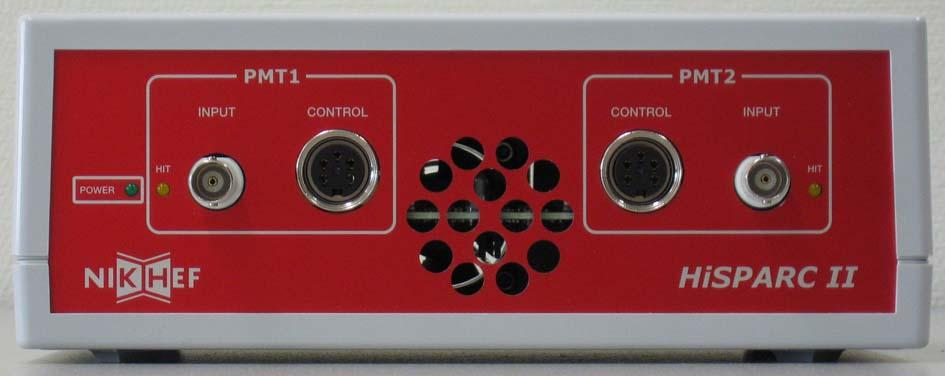
\includegraphics[width=.7\linewidth]{figures/kastje-voorkant}
\caption{\captitle{Front of the HiSPARC II electronics} with connectors for the
PMT control and signal cables for two channels.}
\label{fig:electronics-box}
\end{figure}
\begin{figure}
\centering
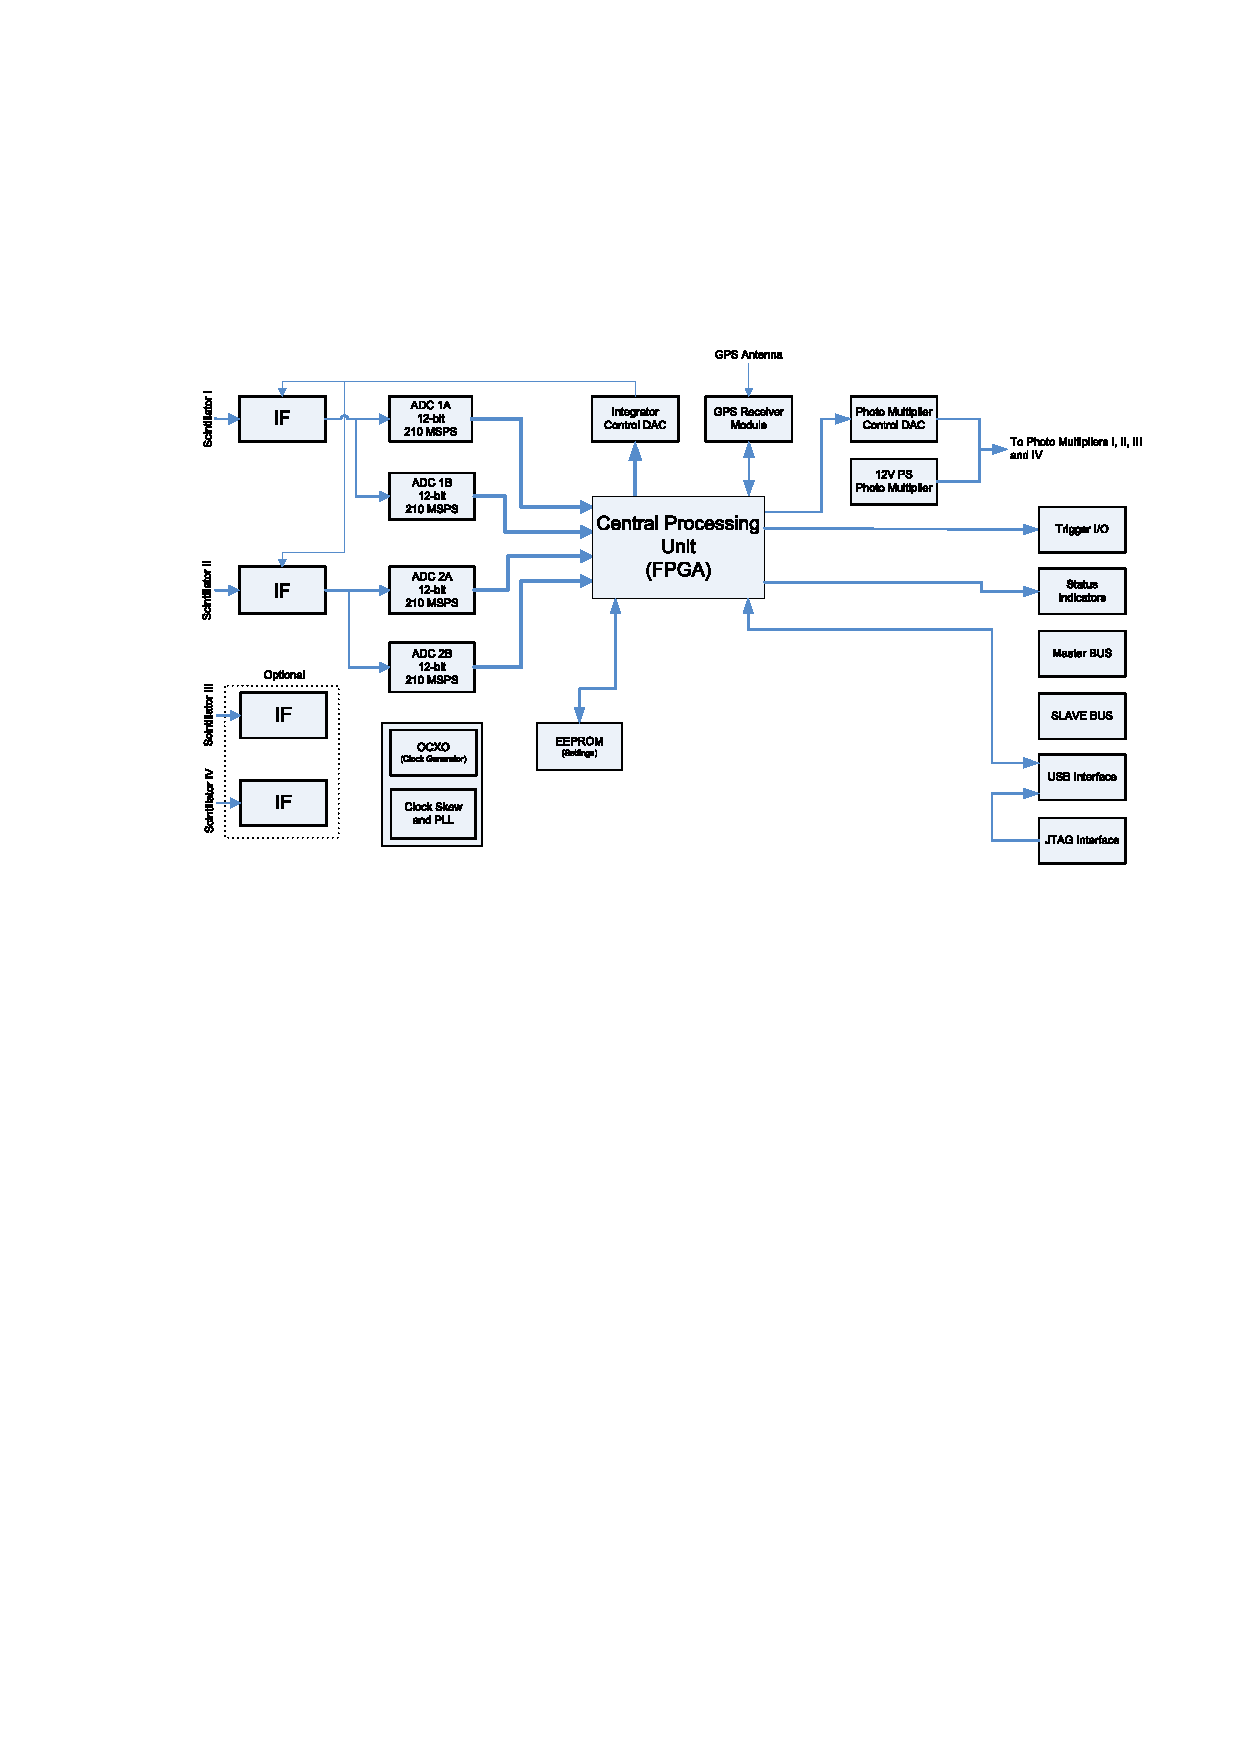
\includegraphics[width=\linewidth]{figures/electronics-schematics}
\caption{Overview of the \hisparc electronics components. Each analog PMT
signal is digitized by two ADCs and the digital signals are fed into the central
processing unit, which is implemented in a FPGA. The FPGA communicates with the
GPS unit and the PC. The trigger and PMT voltage control are also implemented in
the FPGA.
On power up, the EEPROM contents are used to initialize the FPGA. The EEPROM
itself can be flashed using the on-board JTAG interface.}
\label{fig:electronics-schematics}
\end{figure}
The unit is connected to the station PC using a USB 1.1 interface. The \daq
consists of a total of four AD converters to digitize the analog signal from two
PMTs. Thus, two ADCs are used per channel. The electronics contains a
\SI{200}{\mega\hertz} crystal to drive the ADCs. By clocking one ADC at the
rising edge of the clock, and one ADC at the falling edge, the signal can be
sampled with \SI{400}{\mega\hertz}, i.e. a sampling time of only
\SI{2.5}{\nano\second}. This way, the samples from the signal are alternately
provided by the two converters. This requires that the ADCs be carefully
aligned. If the baselines are not carefully aligned, a ragged signal will result
(resembling a triangular wave). This alignment procedure can be carried out by
the user after installation of the station and is performed by applying several
different internal reference voltages on the input channel.  The ADC gains and
offsets can be controlled by software and are adjusted until the ADCs are both
aligned and are providing a sampling range of
\SIrange[retain-explicit-plus]{+113}{-2222}{\milli\volt}. The process is fully
automated and the ADC response is highly linear over this range. The converters
provide a \SI{12}{bit} output, corresponding to a resolution of
\SI{-.57}{\milli\volt} per \adc count.  A conversion of \adc counts to \si{\milli\volt} units is
then given by $V = -.57x + 113$, with $x$ the number of \adc counts.

The trigger logic is implemented in a FPGA module. The firmware is designed to
communicate with a \emph{slave} module, which is an identical \hisparcii
unit without the GPS board. Each readout unit has its own clock and
information on signal levels are communicated to the master's FPGA. For each
channel, two comparator thresholds can be set: the \emph{low threshold}, and the
\emph{high threshold}. The trigger conditions can be set as follows: the number
of required channels over the low threshold, AND or OR the number of required
channels over the high threshold. For example, the default trigger condition
for a four-detector station is 3 low OR 2 high signals, with the
thresholds set at \SI{-30}{\milli\volt} and \SI{-70}{\milli\volt}. This means that over all four channels, at least 3
signals higher than \SI{-30}{\milli\volt} will result in a trigger.
Additionally, two signals higher than \SI{-70}{\milli\volt} will also generate a
trigger. Once a trigger occurs, the master unit instructs the slave unit to
store and send the event messages to the station PC.

For each event, the maximum time frame is \SI{10}{\micro\second}, which is equal
to \num{4000} samples.  Each sample is \SI{12}{\bit}, i.e.
\SI{1.5}{\byte}.  Since the electronics has two channels, the total size of an
event is \SI{12}{\kilo\byte}.  If a trigger is generated, the event is kept in a
buffer (\SI{36}{\kilo\byte}),
waiting for transfer to the PC over the USB connection.  If the buffer has
insufficient space to store a new event, the new event is discarded.  USB 1.1
has a specified data rate of \SI{12}{\mega\bit\per\second}. Theoretically, this
would allow for a trigger rate of up to \SI{125}{\hertz}. Since the Windows
operating system is not a real-time OS, the USB buffers are polled. The
frequency with which this polling is done reduces the maximum attainable trigger
frequency substantially (typically $\sim \SI{30}{\hertz}$).

By default, the pre-trigger window is set to
\SI{1}{\micro\second}, the coincidence window to \SI{1.5}{\micro\second} and the
post-trigger window to \SI{3.5}{\micro\second}, making a total of
\SI{6}{\micro\second}.  In this configuration, the event buffer can hold up to
five events, and the maximum attainable trigger rate increases.
